% *********************************************************************
% © 2026 Jeremy Sylvestre
%
% Permission is granted to copy, distribute and/or modify this document
% under the terms of the GNU Free Documentation License, Version 1.3 or
% any later version published by the Free Software Foundation; with no
% Invariant Sections, no Front-Cover Texts, and no Back-Cover Texts. A
% copy of the license is included in the appendix entitled “GNU Free
% Documentation License” that appears in the output document of this
% PreTeXt source code. All trademarks™ are the registered® marks of
% their respective owners.
%
% *********************************************************************
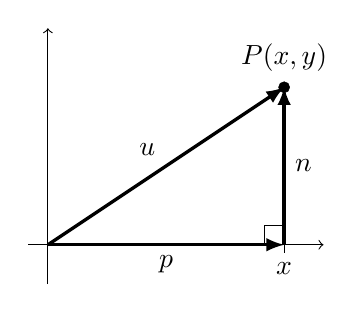
\begin{tikzpicture}[
	vector/.style={-latex,very thick},
	point/.style={circle,draw,very thin,fill,inner sep=0pt,minimum size=4pt},
	% scale=0.75
]
	\coordinate (o) at (0,0);
	\coordinate (p) at (3,2);
	\coordinate (foot) at (3,0);

	\draw[->] (-0.25,0) to (3.5,0);
	\draw[->] (0,-0.5) to (0,2.75);

	\node[point] at (p) [label=above:{$P(x,y)$}] {};
	\draw[thin] (3,0.1) to (3,-0.1) node[below] {$x$};

	\draw[vector] (o) to node[above left] {$\uvec{u}$} (p);
	\draw[vector] (o) to node[below] {$\uvec{p}$} (foot);
	\draw[vector] (foot) to node[right] {$\uvec{n}$} (p);

	% perp symbol
	\begin{scope}[xshift=3cm]
		\draw[thin] (-0.25,0) to (-0.25,0.25) to (0,0.25);
	\end{scope}

\end{tikzpicture}
